\usepgfplotslibrary{colorbrewer}
\usetikzlibrary{calc}

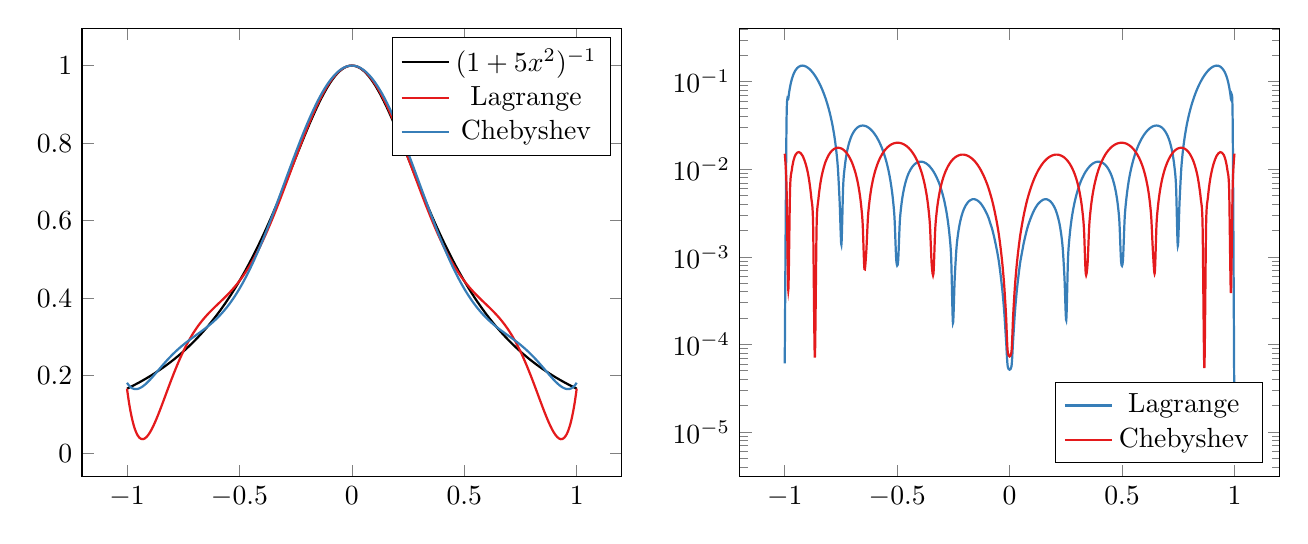
\begin{tikzpicture}
\pgfplotsset{cycle list/Set1-4}
\begin{axis}[name=plot1,
             smooth,
             domain=-1:1,
             samples=255,
             cycle multi list={Set1-4}]

 \addplot+[black, thick] {(1 + 5*x^2)^-1};
 \addlegendentry{$(1+5x^2)^{-1}$};

 \pgfplotsset{cycle list shift=-1} 

 \addplot+[thick] {1 + x^2 * (-35305/7686 + x^2 * (474050/34587 + x^2 * (-664000/34587 + (320000*x^2)/34587)))};
 \addlegendentry{Lagrange}

 \addplot+[thick] {1 + x^2 * (-144680/34561 + x^2 * (348400/34561 + x^2 * (-392000/34561 + (160000*x^2)/34561)))};
 \addlegendentry{Chebyshev}
  
\end{axis}

\begin{semilogyaxis}[name=plot2, at={($(plot1.east) + (1.5cm, 0)$)}, anchor=west,
    smooth,
             domain=-1:1,
             samples=255,
             cycle multi list={Set1-4}, legend pos=south east]

 \addplot+[thick] {abs( (1 + 5*x^2)^-1 - (1 + x^2 * (-35305/7686 + x^2 * (474050/34587 + x^2 * (-664000/34587 + (320000*x^2)/34587)))))};
 \addlegendentry{Lagrange}

 \addplot+[thick] {abs( (1 + 5*x^2)^-1 - (1 + x^2 * (-144680/34561 + x^2 * (348400/34561 + x^2 * (-392000/34561 + (160000*x^2)/34561)))))};
 \addlegendentry{Chebyshev}
\end{semilogyaxis}

\end{tikzpicture}
